%auto-ignore

\section{Evaluation}
\label{sec:results}

We evaluate \this{} along three axes: its success in statically enforcing PM
safety properties, its ease of use, and its performance.

\subsection{Static Checking}

\This{} aims to make the programmer's life easier by statically enforcing PM safety at compile time rather than relying on dynamic checks and testing to identify bugs.
To measure its success in this regard, we
compare it with other PMEM programming systems.

\reftab{tab:libs} summarizes how \this{} and other PM libraries detect violations of
\this{}'s six design goals.  In the table, ``S'' (for ``Static'') means that the compiler
either enforces the invariant automatically (e.g., by generating safe code) or detects any violations and
reports them, ``D'' (``Dynamic'') means that the system will identify the problem at
runtime and exit appropriately, % \steve{not always exits: V-to-NV returns a Result which without panic. If you unwrap the Result, then it panics.}
and ``M'' (``Manual'') means that the system does not detect
violations, so they will manifest as a crash, data corruption, or
other error.  For \nameref{goal:no-memory-leaks}, ``GC'' means the system
provides garbage collection.

The table shows that \this{} enforces almost all its invariants at compile
time, compared to the relatively few compile-time checks other systems provide.

In some cases, this difference represents a design trade-off.  For instance,
NVM Direct explicitly supports unlogged stores as performance optimization.
Likewise, four of the systems allow unsynchronized access which is faster but
less safe.  A \this{} programmer could use similar techniques to improve
performance with \csym{unsafe}.


\begin{table}
  \footnotesize
  \center
  \begin{tabular}{|r||c|c||c|c|}
    \hline
    & Rust & \This{} & C++ & PMDK \\ \hline\hline
    Linked List & 192&+19 (9.9\%) & 146&+45 (30.8\%)  \\ \hline
    Binary tree & 256&+12 (4.7\%) & 208&+41 (19.7\%) \\ \hline
    HashMap     & 165&+10 (6.1\%)  & 137&+42 (30.7\%) \\ \hline
  \end{tabular}
  \caption{Adding persistence to data structures with \this{} requires fewer
    changes (measured in lines of code) than PMDK.}
  \label{tab:loc}
\end{table}

\subsection{Ease of Use}
\label{sec:ease}

A key goal of \this{} is to make writing safe persistent memory programs
easier.  Qualitatively, we would expect that the stronger static guarantees
that \this{} provides should lead to less debugging.  This is especially
valuable since many of the bugs that \this{} protects against would manifest
during a failure, making them more difficult to test.  Our experience using
\this{} bears this out: once code compiles, it works reliably.  
Getting the code to compile can take a while.

\ignore{
Achieving this is a balancing act: On the one hand, \this{} provides
must stronger safety guarantees that existing PMEM libraries.  This should
reduce the number of bugs and vastly increase programmer confidence that their
code is reliable and correct.  Rust's popularity in the system programming
world demonstrates the value of this approach.

On the other hand, \this{} requires programmers to use Rust, a language that
presents a daunting learning curve and, if you are a C or C++ programmer, the
challenges of cross-language integration.

Consider how this trade-off might play out for an experienced C or C++
programmer who wants to write their first PMEM program.  They could pickup
PMDK~\cite{pmdk} and create persistent data structure relatively quickly, but
they would (or should) have only modest confidence that the structure would
crash consistent and thread safe.  It is likely that their first attempt missed
important corner cases.  With practice, debugging, and careful thought, they
would eventually fix the problems and deliver a working, reliable structure.

Alternately, they could learn Rust and then use \this{} to build the same data
structure.  They would likely find that Rust presents a significant and
sometimes frustrating learning curve.  The pay off is that there are no
segmentation faults and, quite often, if the code compiles, it works.

Adding \this{} presents additional typing complexity and more fighting with the
compiler.  However, once the code compile, it is likely to work, and the
guarantees that \this{} provides provide great confidence that the PM-specific
aspects of the code are correct as well.  This is especially valuable since
bugs in these aspects of the program only manifest during recovery, making them
hard to test.
}
%% Adding \this{} presents additional typing complexity.  Getting
%% the code to compile resembled a series of type checking puzzles.  They were
%% challenging -- perhaps just as hard as carefully checking PMEM code -- but
%% relying on the type checker for correctness removed the anxiety of wondering
%% whether a corner case had been missed.  Again, once the code compile, it
%% generally worked.  Further, because of the guarantees that \this{} provides,
%% the programmer could be confident that the PM-specific aspects of the code were
%% correct as well.  This is especially valuable since bugs in these aspects of
%% the program only manifest during recovery, making them hard to test.


Quantitatively, we can measure programing effort by lines of code needed to add
persistence to a conventional program.  We implemented three data structures in
C++ and Rust and then added persistence using PMDK and \this{}. \reftab{tab:loc} shows
that \this{} required adding fewer lines in both relative and absolute terms.


\ignore{This task is challenging and time consuming.  However, since
\this{} checks many key properties statically, once the code compiles they can
have much higher confidence its crash consistency and thread safety.


While we have not performed a formal user study, the authors' experience with
\this{} provide some perspective on its strengths.  One of the authors (an
experienced C/C++ and PM programmer) had not used Rust.  Over the course of a
week or so they learned Rust and then \this{} by building simple volatile and
then persistent data structures.




The authors' experience using \this{} followed 

\This{} aims to make persistent programming easier for Rust programmers by
making it more difficult to write buggy code.  It also aims to match common
Rust programming conventions, so that

Ease of use is the key advantage of \this{}. Persistent libraries are competing
each other over this metric to provide safe programming environment without
requiring the programmer to be an expert in persistent
programming~\cite{pmdk,nvheaps,atlas,javapersistence}.  Using Rust's standard
programming style, we implement \this{} in an idiomatic and familiar way to
make its usage as simple as possible. For instance, the smart pointers in
\this{} act similar to their volatile cousins.  Additionally, shifting
the persistence bugs to the compile time allows debugging at almost zero cost.

}

% To grasp a sense of differentiation between standard programming in Rust and persistent programming with \this{}, \reflst{lst:reimpl} re-implements the same function in \reflst{lst:mut} in volatile memory.

% \begin{lstlisting}[caption={Reimplementation of \reflst{lst:mut} using std crate},label={lst:reimpl}]
% type Ptr = 
%     Option<Rc<RefCell<Node> > >;
% struct Node { val: i32, next: Ptr }
% struct List { tail: Ptr, length: i32 }
% fn add_element(
%     list: &Rc<RefCell<List> >, 
%     val: i32) {
%     panic::catch_unwind(
%     AssertUnwindSafe(move ||{
%         let mut list = list.borrow_mut();
%         list.tail = Some(Rc::new(
%             RefCell::new(Node{
%                 val, next: Null
%             })));
%         list.length += 1;
%     })).expect("Unsuccessful");
% }
% \end{lstlisting}

% As shown above, except the transaction block which is replaced with a \csym{catch\_unwind()}\footnote{\csym{catch\_unwind()} can be seen as a try-catch block which catches the exception arisen inside the closure.} section and \csym{Journal} object passing, everything else is exactly similar to standard Rust programming while using \csym{Rc<RefCell<T>{>}} instead of \csym{Prc<LogRefCell<T,P>,P>}. This shows how idiomatic \this{} would be for Rust programmers with minimal knowledge of persistent programming. Note that, because there is no rollback mechanism in standard Rust for volatile objects, interior mutability is not allowed in \csym{catch\_unwind} section. Therefore, the programmer takes the risk of undesirable changes by asserting that the closure does not panic. However, Rust recommends not having an unwind catching section with mutable references for memory safety.


\subsection{Evaluation Platform}
\label{sec:res:platform}

Our test platform has dual 24-core Cascade Lake processors.  The CPUs are
engineering samples with specs similar to the Xeon Platinum 8160.  In total, the
system has 384~GB (2 socket × 6 channel × 32~GB/DIMM) of DRAM, and 3~TB (2
socket × 6 channel × 256~GB/DIMM) of Intel Optane DC DIMMs.  Our machine runs Fedora 27 with
Linux kernel version 4.13.0.

\This{} uses some unstable features of Rust, so we use Rust Nightly version
1.45.0 built with `release' profile.  We compared \this{} with PMDK 1.8 built
with `-O2'.  We use \extfsDAX{} to mount the persistent memory and create the
pool files.

\ignore{\subsection{Testing}
\label{sec:res:qoality}

For QoS, we focus on the crash consistency of data, and there are no metrics to show that other than the quality of being \textit{correct} or \textit{incorrect}. One single \textit{incorrect} situation infers the low quality of the design. \this{} is verified through a series of intensive workload with the presence of possible thread failure. Note that we cannot emulate real power failure since it was not possible to physically unplug the server. Therefore, the write ordering remains untested, while the logging system is verified through manually killing the process, rerunning it, and comparing the results.

\subsubsection{Methodology}
\label{sec:res:qoal:method}

In this experiment, we developed a set of inductive workloads producing progressive results: the output of the process at time $t+1$ depends on the output of the process at time $t$. To fairly test the correctness, a separate process generates \csym{SIGKILL} randomly and kills the running process. Thus, the possibility of crashing is the same at every point of execution. A crash may happen while working with data, taking log, allocating memory, etc. The final results are compared with the normal execution of the program.

% \begin{table}
% \center
% \small
% \caption{Crash consistency workloads}
% \label{tab:qoal:wrkld}
% \begin{tabular}{|p{0.5in}|p{2.5in}|}
%     \hline
%     FFT {\scriptsize (Single-Thread)} & Calculating FFT of a signal of 1000 samples \\ \hline
%     Fibo {\scriptsize (Multi-Pool)} & Calculating the 1000th item of the Fibonacci series. It keeps the last two numbers in two different pools. A chaperoned session is used to atomically update both numbers. \\ \hline
%     Grep {\scriptsize (Multi-Thread)} & MapReduce implementation of a word counter program that finds the frequency of all words in a list of files. Two threads read from file and push string lines with at-least 1024 characters in a shared stack. Another 16 threads pop from the stack, count the words, and update a shared \csym{HashMap} mapping words to their frequency in three separate transactions.  \\ \hline
% \end{tabular}
% \end{table}
}

\ignore{\subsubsection{Workloads}
\label{sec:res:qoal:workload}

% \reftab{tab:qoal:wrkld} shows the three micro-benchmarks we used to verify single-thread thread programs, chaperoned multi-pool programs, and multi-thread persistent objects. 
We implemented three micro-benchmarks to verify single-thread thread programs, chaperoned multi-pool programs, and multi-thread persistent objects, respectively. 
\textit{FFT} performs a fast fourier transform of a signal with 1000 samples. The root object of FFT contains the input and out put lists of samples, the counters of two nested loops, and some other persistent parameters. In case of a crash, it recovers to the latest consistent state and continues iterating over the samples from there. The \textit{Fibo} benchmark calculates the 1000th element in the Fibonacci series. We used two separate pools to verify cross-pool atomicity in this example. One pool contains $fibo[n]$ and the other one contains $fibo[n-1]$. On every iteration, the value of $fibo[n]$ updates to $fibo[n]+fibo[n-1]$ in one transaction, and $fibo[n-1]$ becomes the old value of $fibo[n]$ in another transaction, both are handled in a chaperoned session. When a crash happens, both transactions roll back to their consistent states, and the process continues from there. The last test is \textit{Wordcount} which takes a regular expression pattern and counts the captured matches and update a shared hash map. The recovery procedure in this case releases the locks and reverts the uncommitted changes.

The experiments reveal that the final output of the applications with the possibility of crashes are consistent with the output of the normal execution in all of the mentioned scenarios. The memory usage in all cases also does not change which confirms the reliability of \this{}'s memory management.
}
\subsection{Performance}
\label{sec:res:perf}

We compared our library with PMDK's libpmemobj and libpmemobj++ by porting some PMDK data structures to \this{}.  

\ignore{\subsubsection{Methodology}
\label{sec:res:qoal:method}

To measure the performance in both \this{} and PMDK, we use the linux provided tool \csym{perf}. We use \extfsDAX{} to mount the persistent memory and create the pool files in both cases in the same location. To fairly compare the performance, we use the same CPU mask for both cases, and run the experiments on the local NUMA node. Both libraries are built at the same (equivalent) level of optimization.}

\begin{table}
      \center
      \footnotesize
    \begin{tabular}{|p{0.5in}|p{2.5in}|}
        \hline
        BST & A transaction-free and failure-atomic implementation of a Binary Search Tree \\ \hline
        KVStore & A simple Key-Value store data structure using hash map \\ \hline
        B+Tree & An optimized, balanced B+Tree with 8-way fanout.  \\ \hline
        wordcount & Counts the occurrences of each word in a corpus of text using a hashmap and producer/consumer threads\\\hline
    \end{tabular}
    \caption{Microbenchmarks. The first three are used to compare the performance of \this{} with PMDK. Wordcount measures \this{}'s scalability with thread count.}
    \label{tab:perf:wrkld}
\end{table}

%(Only on \this{}) A MapReduce implementation of a word counter pro-gram  that finds  the  frequency  of all words  in  alist of files.  Two threads read from file and pushstring lines with at-least 1024 characters in a sharedstack. Another 16 threads pop from the stack, countthe words, and update a sharedHashMapmappingwords to their frequency in three separate transac-tions. \\ \hline

\subsubsection{Workloads}
\label{sec:res:perf:workload}

\reftab{tab:perf:wrkld} summarizes the workloads we used to evaluate the performance of \this{} and its scalability.  The first three applications are used to compare performance with PMDK. The PMDK version of BST, KVStore, and B+Tree are available in PMDK repository.   We reimplemented them in \this{} using the same algorithms.

% The BST data structure consists of nodes that are wrapped in \csym{MaybeNull<Pbox<\_>{>}}. Since there is no data sharing and moving nodes, we use \csym{Pbox}. To atomically allocate new nodes without transactions, we leverage the low-level atomic allocation provided in \csym{MaybeNull::initialize()} function. This function is specialized for pointer type wrappers. Taking the inner data of type \csym{T} to be located in the PM, it returns an instance of \csym{Valid(Pbox<T>)} only if the old value was \csym{Null} (otherwise, raises an error). The performance of \csym{initialize} is comparable with \csym{POBJ\_ALLOC} in PMDK, but it works with safe data. We measure the performance of inserting 30,000 integers (INS) and checking their presence (CHK) in the data structure.

% The KVStore workload uses a hash map data structure in which keys are of type  persistent string, and values are 64-bit integers. Key-Value pairs are organized in 10 vectors as buckets. The structure should be able to update the value when the key already exists. Therefore, we use \csym{LogRefCell} to be able to update values.%Since we are using persistent vectors belonging to the root object, there is no need to have pointers. New data are pushed to the persistent vectors directly. Variable-sized vectors are also wrapped in \csym{LogRefCell} to provide guarded mutability while putting new data.
% We measure the performance of putting 100,000 uniquely named key-value pairs (PUT) and retrieving all of them (GET).

% The B+Tree implementation is more complicated than the other two as it self-balance while operating. Since data might move from one node to another, we use \csym{Prc} to be able to move pointers to data between nodes without moving data itself.
% Each node consists of two fixed size arrays of items and children slots. To allow safe mutable access to the arrays, each node is wrapped in a \csym{Prc<LogRefCell<\_>{>}}. 
% We measure the performance of inserting 1,000,000 uniquely randomized values stored in a file (INS), checking their presence (CHK), removing all of them one-by-one (REM), and random operations (RAND) with the same input for both PMDK and \this.

% The Grep workload is only implemented in \this{} to measure its scalability to the number of threads. It takes a pattern and a list of files; then, it finds all matches and their frequency in all files. We use MapReduce design to implement Grep: $p$ threads produce feeds for another $c$ threads to consume them.
%There are $p$ number of producer threads which read chunks of lines from the given files and atomically put them to a shared stack list. At the same time, $c$ number of consumer threads pop from the stack and buffer the chunks in their own local persistent buffers in one transaction; then, they count the number of captured matches and updated their local persistent hash table with their frequency in another transaction; finally, they updated the shared hash table with their local data in a third separate transaction. We used persistent buffers to allow resumable process when crash happens. 
% The workload reads two separate large text files with the total number of 1,092,186 words (33,855 distinct words) and produces a map from words to their frequencies.

%http://corpus.canterbury.ac.nz/descriptions/

\subsubsection{Results}
\label{sec:res:perf:res}

\reffig{fig:perf} shows the results of our experiments comparing \this{}'s performance with PMDK and \this{}-dynamic, a version of \this{} that does not use pool types, but instead relies on dynamic checks to achieve design goal 2 (\nameref{goal:ptrs-are-safe}).

Performance with pool types (``\this{}'') is always at least as fast as PMDK,
and sometimes significantly faster.  Dynamic checks (\this{}-Dynamic)
hurt performance since they require (at least) obtaining the pool object and
performing several comparisons.

\begin{figure}
    \begin{center}
    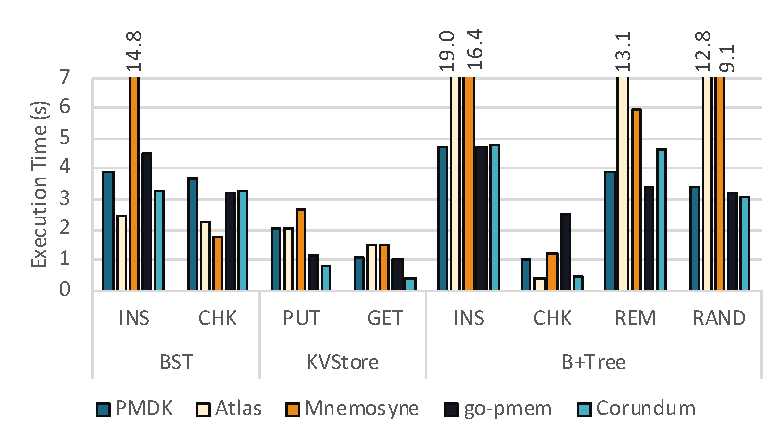
\includegraphics[width=3.3in]{Graphs/perf.pdf}
    \end{center}
    \caption{\label{fig:perf} Performance comparison between \this{} and PMDK}
\end{figure}

Wordcount measures scalability.  \This{} provides
%\steve{separate allocators for every core, and (I changed it back to single allocator to prevent some sync issues when one allocator is full. It was easier to debug. Anyway, it didn't destroy the performance, at all.)}
a separate journal object for every thread to allow concurrency. %concurrent allocation.
\reffig{fig:scal} confirms that the performance scales with thread count.  The bottleneck in this experiment is the contention over the shared data structures that threads use to communicate.

\begin{figure}
    \begin{center}
    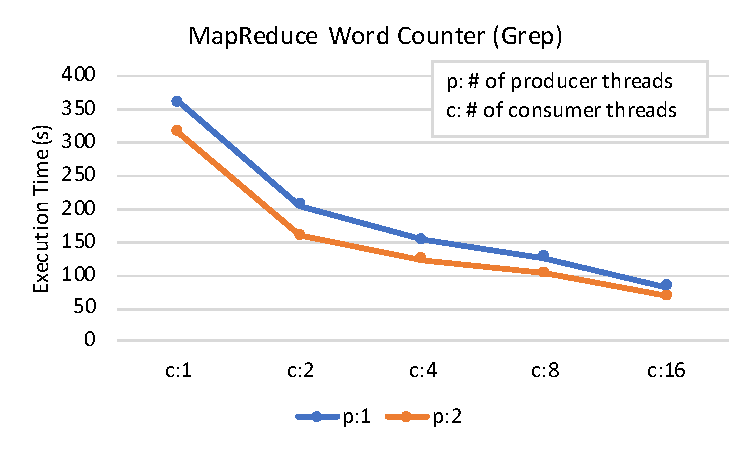
\includegraphics[width=3.3in]{Graphs/scal.pdf}
    \end{center}
    \caption{\label{fig:scal} \this{}'s scalable performance with regard to the number of threads}
\end{figure}
